%CHAPTER 6
\chapterfigure[width=\linewidth]{Durer/Durer_Revelation_Four_Riders.jpg}[The Four Horsemen]{The Four Horsemen. Albrecht Dürer, 1498.}

\chapter{The First Six Seals}
\fancyhead{} %clear formatting
\fancyhead[LE]{CHAPTER 6} %for even pages, put the chapter number on left side; for odd pages, put chapter title on right
\fancyhead[RO]{THE FIRST SIX SEALS}
\subsubsection*{The First Seal}
\lettrine[lines=3]{\textcolor{red}{A}}{\ nd I saw when the Lamb opened} one of the seven seals, and I heard one of the four living creatures saying as with a voice of thunder, Come. 
\vnum{2}And I saw, and behold, a white horse,%
	\cbiblefootduosb{Zechariah}{1:8-11}{I saw in the night, and, behold, a man riding upon a red horse, and he stood among the myrtle-trees\ldots\ and behind him there were horses, red, sorrel, and white\ldots\ And the man that stood among the myrtle-trees\ldots\ said, These are they whom Jehovah hath sent to walk to and fro through the earth. And they answered the angel of Jehovah\ldots\ We have walked to and fro through the earth, and, behold, all the earth sitteth still, and is at rest.}%
					{6:1-8}{There came four chariots out from between two mountains\ldots\ In the first chariot were red horses; and in the second chariot black horses; and in the third chariot white horses; and in the fourth chariot grizzled strong horses\ldots\ These are the four winds of heaven, which go forth from standing before the Lord of all the earth\ldots\ and he said, Get you hence, walk to and fro through the earth.} %
and he that sat thereon had a bow; and there was given unto him a crown: and he came forth conquering, and to conquer.
\subsubsection*{The Second Seal}
\vnum{3}And when he opened the second seal, I heard the second living creature saying, Come. %
\vnum{4}And another horse came forth, a red horse: and to him that sat thereon it was given to take peace from the earth, and that they should slay one another: and there was given unto him a great sword.
\subsubsection*{The Third Seal}
\vnum{5}And when he opened the third seal, I heard the third living creature saying, Come. And I saw, and behold, a black horse; and he that sat thereon had a balance in his hand. %
\vnum{6} And I heard as it were a voice in the midst of the four living creatures saying, A measure of wheat for a shilling, and three measures of barley for a shilling; and the oil and the wine hurt thou not.
\subsubsection*{The Fourth Seal}
\vnum{7}And when he opened the fourth seal, I heard the voice of the fourth living creature saying, Come. %
\vnum{8}And I saw, and behold, a pale horse: and he that sat upon him, his name was Death; and Hades followed with him. And there was given unto them authority over the fourth part of the earth, to kill with sword, and with famine, and with death, and by the wild beasts of the earth.%
	\footnote{\cbibleref{Ezekiel}{5:12, 17}{A third part of thee shall die with the pestilence, and with famine shall they be consumed in the midst of thee; and a third part shall fall by the sword round about thee; and a third part I will scatter unto all the winds, and will draw out a sword after them\ldots\ I will send upon you famine and evil beasts, and they shall bereave thee; and pestilence and blood shall pass through thee; and I will bring the sword upon thee: I, Jehovah, have spoken it} %
			\cbiblechvs{Ezekiel}{14:21}{How much more when I send my four sore judgments upon Jerusalem, the sword, and the famine, and the evil beasts, and the pestilence, to cut off from it man and beast!} %
			\cbiblechvs{Ezekiel}{33:27}{Thus saith the Lord Jehovah: As I live, surely they that are in the waste places shall fall by the sword; and him that is in the open field will I give to the beasts to be devoured; and they that are in the strongholds and in the caves shall die of the pestilence.} %
			\cbibleref{Jeremiah}{14:12}{ I will consume them by the sword, and by the famine, and by the pestilence} %
			\cbiblechvs{Jeremiah}{15:2-3}{Thus saith Jehovah: Such as are for death, to death; and such as are for the sword, to the sword; and such as are for the famine, to the famine; and such as are for captivity, to captivity. And I will appoint over them four kinds, saith Jehovah: the sword to slay, and the dogs to tear, and the birds of the heavens, and the beasts of the earth, to devour and to destroy.}
			}%
\subsubsection*{The Fifth Seal}
\vnum{9}And when he opened the fifth seal, I saw underneath the altar the souls of them that had been slain for the word of God, and for the testimony which they held: %
\vnum{10}and they cried with a great voice, saying, How long, O Master, the holy and true,%
	\cbiblefootduo{Psalms}{79:1-6}{O God, the nations are come into thine inheritance; thy holy temple have they defiled\ldots\ The dead bodies of thy servants have they given to be food unto the birds of the heavens, the flesh of thy saints unto the beasts of the earth. Their blood have they shed like water\ldots\ and there was none to bury them\ldots\ How long, O Jehovah? Wilt thou be angry for ever? Shall thy jealousy burn like fire? Pour out thy wrath upon the nations that know thee not, and upon the kingdoms that call not upon thy name.}%
				{Zechariah}{1:12}{O Jehovah of hosts, how long wilt thou not have mercy on Jerusalem and on the cities of Judah, against which thou hast had indignation these threescore and ten years?} %
dost thou not judge and avenge our blood on them that dwell on the earth?%
 	\footnote{\cbibleref{Psalms}{79:10-13}{Wherefore should the nations say, Where is their God? Let the avenging of the blood of thy servants which is shed be known among the nations in our sight\ldots\ Preserve thou those that are appointed to death; and render unto our neighbors sevenfold into their bosom their reproach, wherewith they have reproached thee, O Lord. So we thy people and sheep of thy pasture will give thee thanks for ever: we will show forth thy praise to all generations.}} %
\vnum{11}And there was given them to each one a white robe; and it was said unto them, that they should rest yet for a little time, until their fellow-servants also and their brethren, who should be killed even as they were, should have fulfilled their course.
\subsubsection*{The Sixth Seal}
\vnum{12}And I saw when he opened the sixth seal, and there was a great earthquake;%
	\cbiblefoot{Ezekiel}{38:19-20}{In my jealousy and in the fire of my wrath have I spoken, surely in that day there shall be a great shaking in the land of Israel; so that the fishes of the sea, and the birds of the heavens, and the beasts of the field, and all creeping things that creep upon the earth, and all the men that are upon the face of the earth, shall shake at my presence, and the mountains shall be thrown down, and the steep places shall fall, and every wall shall fall to the ground.} %
and the sun became black as sackcloth of hair, and the whole moon became as blood;%
 	\footnote{
 		\cbibleref{Joel}{3:14-16}{The day of Jehovah is near in the valley of decision. The sun and the moon are darkened, and the stars withdraw their shining. And Jehovah will roar from Zion\ldots\ and the heavens and the earth shall shake} %
 		\cbibleref{Isaiah}{13:9-11, 13}{Behold, the day of Jehovah cometh, cruel, with wrath and fierce anger; to make the land a desolation, and to destroy the sinners thereof out of it. For the stars of heaven and the constellations thereof shall not give their light; the sun shall be darkened in its going forth, and the moon shall not cause its light to shine. And I will punish the world for their evil\ldots\ I will make the heavens to tremble, and the earth shall be shaken out of its place, in the wrath of Jehovah of hosts, and in the day of his fierce anger.} %
 		\cbiblechvs{Isaiah}{50:2-3}{Behold, at my rebuke\ldots\ I clothe the heavens with blackness, and I make sackcloth their covering.} % 		
 		\cbibleref{Ezekiel}{32:7-9}{When I shall extinguish thee, I will cover the heavens, and make the stars thereof dark; I will cover the sun with a cloud, and the moon shall not give its light. All the bright lights of heaven will I make dark over thee, and set darkness upon thy land, saith the Lord Jehovah. I will also vex the hearts of many peoples, when I shall bring thy destruction among the nations.}%
 	} %
\vnum{13}and the stars of the heaven fell unto the earth, as a fig tree casteth her unripe figs when she is shaken of a great wind.%
	\cbiblefoot{Isaiah}{34:2-6}{Jehovah hath indignation against all the nations, and wrath against all their host: he hath utterly destroyed them, he hath delivered them to the slaughter\ldots\ And all the host of heaven shall be dissolved, and the heavens shall be rolled together as a scroll; and all their host shall fade away, as the leaf fadeth from off the vine, and as a fading leaf from the fig-tree. For my sword hath drunk its fill in heaven: behold, it shall come down upon\ldots\ the people of my curse, to judgment.} %
\vnum{14}And the heaven was removed as a scroll when it is rolled up; and every mountain and island were moved out of their places.%
	\cbiblefoot{Ezekiel}{26:15}{Thus saith the Lord Jehovah to Tyre: shall not the isles shake at the sound of thy fall, when the wounded groan, when the slaughter is made in the midst of thee?} %
\vnum{15}And the kings of the earth, and the princes, and the chief captains, and the rich, and the strong,%
	\cbiblefootduosb{Isaiah}{24:21}{Jehovah will punish the host of the high ones on high, and the kings of the earth upon the earth}%
					{34:12}{They shall call the nobles thereof to the kingdom, but none shall be there; and all its princes shall be nothing.} %
 and every bondman and freeman, hid themselves in the caves and in the rocks of the mountains;%
 	\footnote{\cbibleref{Isaiah}{2:9-12}{The mean man is bowed down, and the great man is brought low: therefore forgive them not. Enter into the rock, and hide thee in the dust, from before the terror of Jehovah, and from the glory of his majesty. For there shall be a day of Jehovah of hosts upon all that is proud and haughty, and upon all that is lifted up; and it shall be brought low} %
 			\cbiblevs{Isaiah}{2:19-21}{Men shall go into the caves of the rocks, and into the holes of the earth, from before the terror of Jehovah, and from the glory of his majesty, when he ariseth to shake mightily the earth. In that day men shall cast away their idols\ldots\ to go into the caverns of the rocks, and into the clefts of the ragged rocks, from before the terror of Jehovah, and from the glory of his majesty, when he ariseth to shake mightily the earth.}		
 	} %
\vnum{16}and they say to the mountains and to the rocks, Fall on us, and hide us from the face of him that sitteth on the throne, and from the wrath of the Lamb: %
\vnum{17}for the great day of their wrath is come; and who is able to stand?%
	\footnote{
		\cbibleref{Joel}{2:11}{The day of Jehovah is great and very terrible; and who can abide it?} %
		\cbiblechvs{Joel}{3:14}{The day of Jehovah is near in the valley of decision} %
		\cbibleref{Zephaniah}{1:14-15}{The great day of Jehovah is near, it is near and hasteth greatly, even the voice of the day of Jehovah; the mighty man crieth there bitterly. That day is a day of wrath, a day of trouble and distress, a day of wasteness and desolation} %
		\cbibleref{Nahum}{1:6}{Who can stand before his indignation? and who can abide in the fierceness of his anger? His wrath is poured out like fire, and the rocks are broken asunder by him} %
		\cbibleref{Malachi}{3:2}{Who can abide the day of his coming? And who shall stand when he appeareth? For he is like a refiner’s fire, and like fullers’ soap\ldots}%
	}

  \begin{figure*}[p]
  	\centering
  	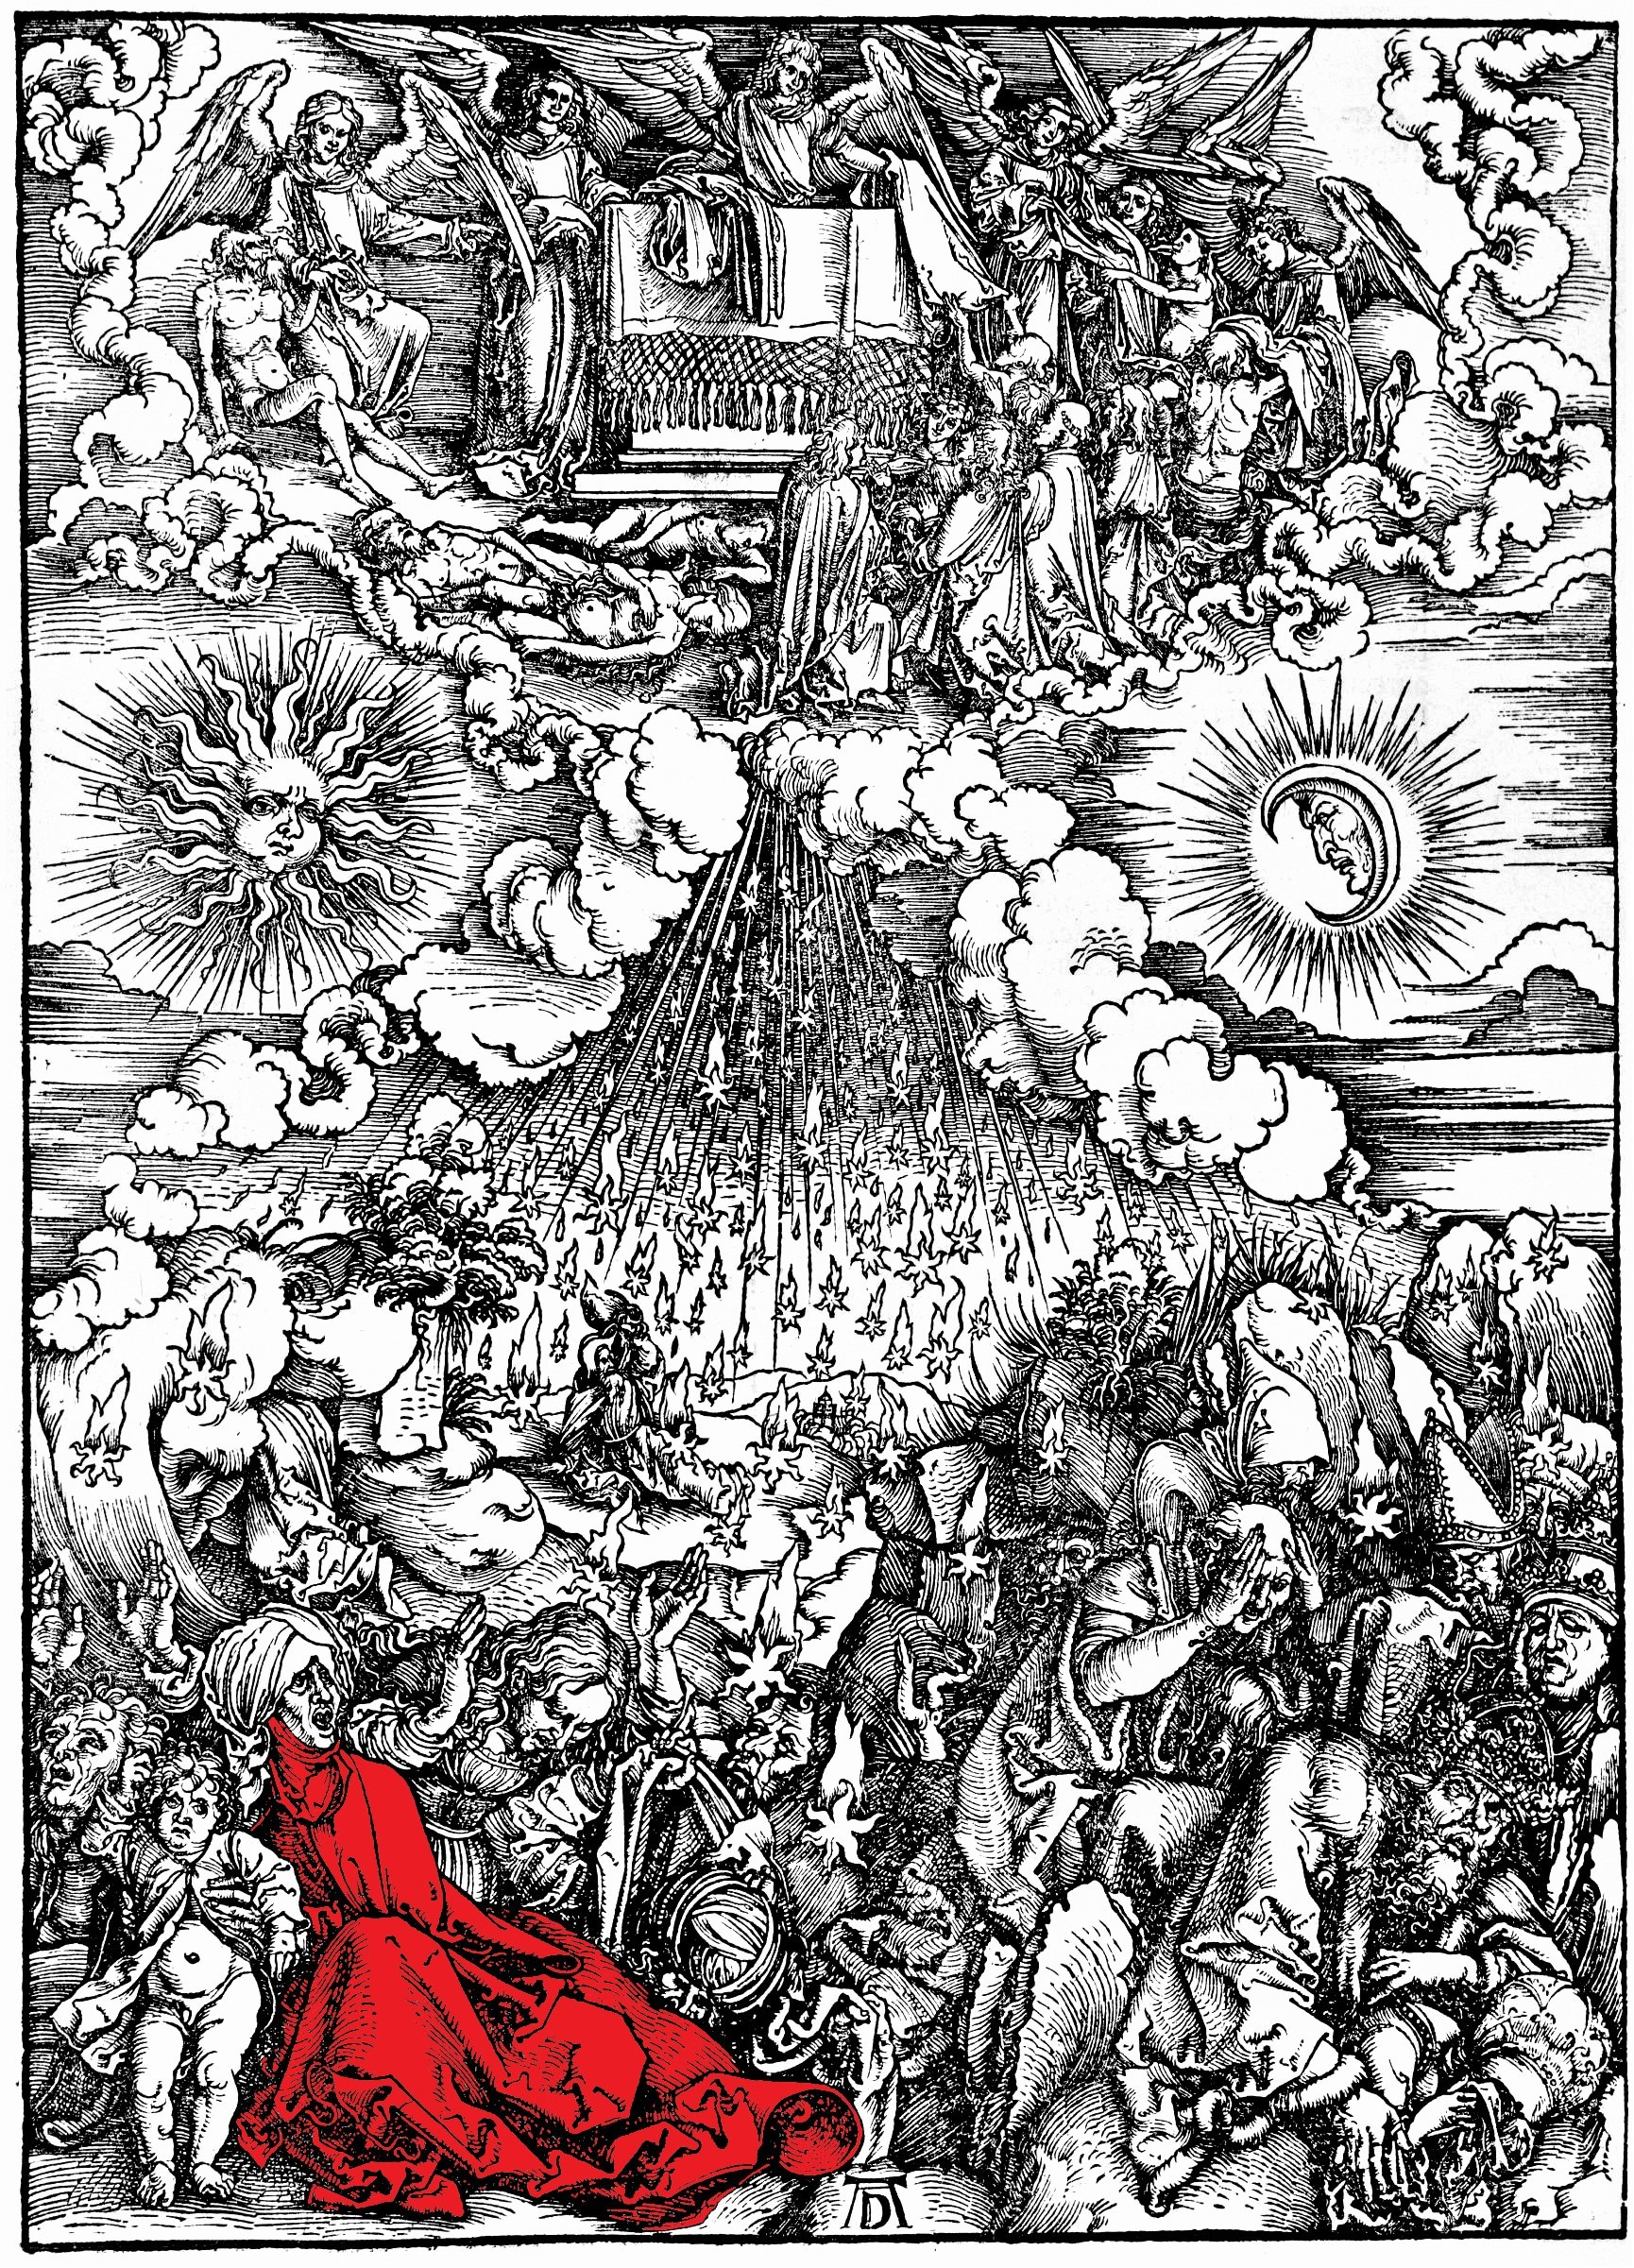
\includegraphics[width=\linewidth]{Durer/Durer_Sixth_Seal.jpg}
  	\caption[The Opening of the Fifth and Sixth Seals]{The Opening of the Fifth and Sixth Seals. Albrecht Dürer, 1498.}
  \end{figure*}
